\documentclass{article}

\usepackage{nips15submit_e,times}
\usepackage{amsmath}
\usepackage{amssymb}
\usepackage{amsthm}
\usepackage{url}
\usepackage{fullpage}
\usepackage{natbib}
\usepackage{subcaption}
\usepackage{graphicx}

\newtheorem{theorem}{Theorem}
\newtheorem{lemma}{Lemma}
\newtheorem{definition}{Definition}

\newcommand{\N}{\mathcal{N}}
\newcommand{\I}{\mathcal{I}}
\newcommand{\R}{\mathbb{R}}
\newcommand{\tr}{\text{tr}}
\newcommand{\eps}{\varepsilon}
\renewcommand{\v}[1]{\mathbf{#1}}

\begin{document}

\title{Gaussian Process Random Fields}
\author{David Moore and Stuart Russell}
\maketitle

\begin{abstract}
Gaussian processes have been successful in both supervised and
unsupervised machine learning tasks, but their cubic complexity has
constrained practical applications. We introduce a new approximation
for large-scale Gaussian processes, the Gaussian Process Random Field (GPRF),
in which local GPs are coupled via pairwise potentials. The GPRF
likelihood is a simple, tractable, and parallelizeable approximation to the full GP marginal
likelihood, enabling hyperparameter selection and latent variable
modeling on large datasets.
\end{abstract}

\section{Introduction}

Many machine learning tasks can be framed as learning a function
given its values at a set of training points. In regression and
classification, these values are observed explicitly; in less-supervised
settings such as latent variable modeling or reinforcement learning,
some aspects of the observations may be available only implicitly. As
a flexible class of probability distributions on functions,  Gaussian
processes (GPs) allow us to approach function-learning problems from
an appealing principled and clean Bayesian perspective.

Unfortunately, practical applications have been constrained by the the cubic time complexity of GP inference with respect
to the number of training points. Exact GP calculations are generally
infeasible for datasets larger than approximately $n=5000$, excluding
many interesting real-world problems. 

Many approximations have been
developed to escape this limitation. One particularly simple approximation is to partition the
input space into smaller blocks, replacing a single large GP with a
multitude of local ones. This gains tractability at the
price of a potentially severe independence assumption. 

In this paper we relax the strong independence assumptions of
independent local GPs, proposing instead a Markov random field (MRF) of
local GPs, which we call a Gaussian Process Random Field (GPRF). The
GPRF couples local models via pairwise potentials that incorporate
covariance information. This yields a surrogate for the full GP
marginal likelihood which is simple to implement and 
can be tractably evaluated and optimized on
large datasets, while still enforcing a smooth covariance
structure. The task of approximating the marginal likelihood is
motivated by unsupervised applications such as the GP latent variable
model \cite{lawrence2004gaussian}, but examining the predictions made by our model also
yields a novel interpretation of the Bayesian Committee Machine \cite{tresp2000bayesian}.

We begin by reviewing Gaussian processes and Markov random fields, and
some existing approximation methods for large-scale GPs. In
Section~\ref{sec:gprf} we present the GPRF objective and examine its
properties as an approximation to the full GP marginal likelihood.  We
then evaluate it on synthetic and real-world datasets, in particular
an application to seismic event location. 

\section{Background}

\subsection{Gaussian processes}
Gaussian processes \citep{rasmussen2006} are
distributions on random functions. A GP is parameterized by a mean function
$\mu_\theta(\v{x})$ and a covariance, or kernel, function $k_\theta(\v{x},
\v{x}')$; these may themselves have hyperparameters $\theta$. Typically we assume the data has been pre-centered so that
we may choose $\mu(\v{x})=0$. A common family of covariances is the squared
exponential, $k_{SE}(\v{x}, \v{x}') =
\sigma^2_f\exp\left(-\frac{\|\v{x}-\v{x}'\|^2}{2\ell^2}\right)$, in
which the hyperparameters $\sigma^2_f$  and $\ell$ specify a prior variance
and correlation lengthscale respectively.

We say that a random function $f(x)$ is Gaussian process distributed if, for
any set of $n$ input points $X$, the vector of function values $\v{f} = f(X)$ is
multivariate Gaussian, $\v{f} \sim \N(\v{0}, k(X, X)).$ In many applications we
have access only to noisy observations $\v{y}$, where we commonly
assume the noise is iid Gaussian, \[\v{y} = \v{f} + \v{\eps},
\qquad \v{\eps}\sim \N(\v{0}, \sigma_n^2 \I).\] In this case the
observations are themselves Gaussian, $\v{y} \sim \N(\v{0}, K_y)$, where $K_y = k_\theta(X, X) + \sigma^2_n\I$. 

Bayesian regression \cite{rasmussen2006} is the most common application of GPs: we attempt to predict the
function at test points $X^*$ via the conditional distribution
$p(\v{f}^* | \v{y}; X, \theta)$ given the training data. Sometimes, however, we do not observe the training inputs $X$, or
observe them only partially or noisily, in which case the standard regression
formulation does not apply. This setting is known as the Gaussian Process
Latent Variable Model (GP-LVM)  \cite{lawrence2004gaussian}; it uses
GPs as a model for unsupervised
  learning and nonlinear dimensionality reduction. GP-LVM
  observations are typically multi-dimensional, $Y = (\v{y}^{(1)}, \ldots,
  \v{y}^{(D)})$, with each dimension $\v{y}^{(d)}$ modeled as an
  independent Gaussian process. The input locations are typically sought via maximization of the {\em marginal likelihood}
\begin{align}
\mathcal{L}(X, \theta) &= \log p(Y ; X, \theta) \nonumber\\
&= \sum_{i=1}^D -\frac{1}{2}\log |K_y| - \frac{1}{2} \v{y}_i^T K_y^{-1} \v{y}_i + C\nonumber\\
&= -\frac{D}{2}\log |K_y| - \frac{1}{2}\tr(K_y^{-1} YY^T) + C,\label{eqn:mlik}
\end{align}
though recent work \citep{titsias2010bayesian,
  damianou2014} attempts to recover a variational posterior. If the
covariance function $k_\theta(\v{x}, \v{x}')$ is differentiable
with respect to $\v{x}$ and/or $\theta$, this maximization can be
performed by gradient-based methods, although care is required in the
initialization as the marginal likelihood is generally non-convex.
Selection of kernel hyperparameters $\theta$, for the pure regression setting and/or the
GP-LVM, can also be accomplished via maximization of $\mathcal{L}$.

\subsection{Scalability and approximate inference}
\label{sec:approx}

\begin{figure}
\centering

\begin{subfigure}[t]{.30\textwidth}
                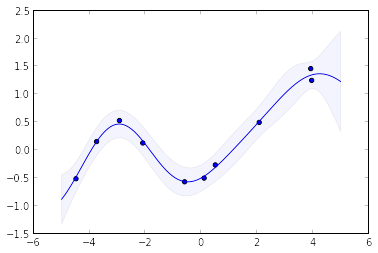
\includegraphics[width=\textwidth]{toy_gp_posterior}
                \caption{Full GP. }
                \label{fig:gp}
        \end{subfigure}
\qquad
\begin{subfigure}[t]{.30\textwidth}
  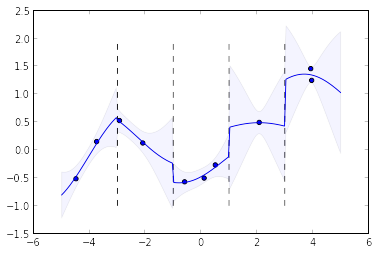
\includegraphics[width=\textwidth]{toy_lgp_posterior}
  \caption{Local GPs.}
  \label{fig:local}
\end{subfigure}
\qquad
\begin{subfigure}[t]{.30\textwidth}
  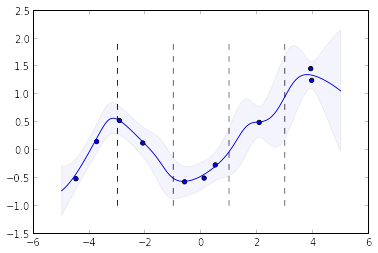
\includegraphics[width=\textwidth]{toy_bcm_posterior}
  \caption{Bayesian committee machine.}
  \label{fig:bcm}
\end{subfigure}
\caption{Predictive distributions on a toy regression problem. The BCM
is operating in its worst-case mode of predicting each test marginal
separately.}
\label{fig:approx}
\end{figure}

The main computational difficulty in Gaussian process methods is
the need to invert or factor the kernel matrix $K_y$, which is cubic
in $n$. In GP-LVM inference this must be done at every optimization step to evaluate
(\ref{eqn:mlik}) and its derivatives.

This complexity has inspired
a number of approximations. The most commonly studied are inducing
point methods, in which the unknown functions are
represented by their values at a small set of $m$ inducing
points, where $m \ll n$. These points can be chosen by maximizing the marginal
likelihood in a surrogate model \citep{quinonero2005, lawrence2007learning} or by
minimizing the KL divergence to the full GP
\citep{titsias2009variational}. Inference in these models can
typically be done in $O(nm^2)$ time, but this comes at the price
of reduced representational capacity: while smooth functions with long lengthscales may
be compactly represented by a small number of inducing points, for
quickly-varying functions with significant local
structure it may be difficult to find any representation more compact
than the complete set of training observations.

A separate class of approximations, so-called ``local'' GP methods
\cite{rasmussen2006, nguyen2009model, zhao2011human, park2011domain}, involves
partitioning the inputs into blocks of $m$ points each, then modeling
each block with an independent Gaussian process. If the partition is
spatially local, this corresponds to a covariance function that imposes independence
between function values in different regions of the input
space. Computationally, each block requires only $O(m^3)$ time; the
total time is linear in the number of blocks. Local approximations
preserve short-lengthscale structure, but their harsh independence assumptions can lead to
predictive discontinuities and inaccurate covariances
(Figure~\ref{fig:local}). These assumptions are especially problematic for
GP-LVM inference because the marginal likelihood becomes
non-differentiable at block boundaries. Nonetheless, local GPs sometimes
work very well in practice, achieving comparable results to more
sophisticated methods while requiring only a fraction of the time \cite{chalupka2012}.

The Bayesian Committee Machine (BCM) \cite{tresp2000bayesian} attempts
to improve on independent local GPs by averaging the predictions of
multiple GP experts. The model is formally equivalent to an inducing point model
in which the {\em test points} are the inducing points, i.e., it
assumes that the training blocks are conditionally independent given
the test data. The BCM can yield high-quality predictions that avoid the
pitfalls of local GPs (Figure~\ref{fig:bcm})
\cite{schwaighofer2002transductive}, while maintaining scalability to
very large datasets \cite{deisenroth2015distributed}. However, as a
purely predictive approximation, it is unhelpful in the latent
variable model setting, where we are interested in the likelihood of
our training set irrespective of any particular test data.  The desire
for a BCM-style likelihood approximation was part of the motivation
for this current work; Section~\ref{sec:approx-predict} shows that the GPRF
proposed in this paper can be viewed as such a model. 

Simple building blocks are often combined to create more complex
approximations. 
The PIC approximation \cite{snelson2007} blends a global
inducing-point model with local block-diagonal covariances, 
thus capturing a mix of global and local
structure, though with the same boundary discontinuities as in
``vanilla'' local GPs. A related approach is the use of covariance
functions with compact support \cite{vanhatalo2008} to capture local
variation in concert with global inducing points. \cite{chalupka2012} surveys and compares
several approximate GP regression methods on synthetic and real-world
datasets. 

We also note here the similar title of \cite{zhong2010gaussian}, which uses a {\em
  latent} random field as a prior on locations to a GP-LVM. By
contrast, our work defines a random field decomposition of the outputs
$\v{y}$, and can be combined with any prior on $X$. 

\subsection{Markov Random Fields}

We recall some basic theory regarding Markov random fields
(MRFs), also known as undirected graphical models \cite{koller2009probabilistic}. A pairwise
MRF consists of an undirected graph $(V, E)$, along with {\em node potentials} $\psi_i$ and {\em edge
potentials} $\psi_{ij}$, which define an {\em energy function} 
\begin{equation}
E(\v{y}) = \sum_{i\in V} \psi_{i}(\v{y}_i) + \sum_{(i,j)\in E}
\psi_{ij}(\v{y}_i, \v{y}_j).\label{eqn:mrf}
\end{equation}
Normalizing this energy yields a probability distribution (the ``Gibbs
distribution''), $p(\v{y}) = \frac{1}{Z}\exp(-E(\v{y}))$, where $Z = \int \exp(-E(\v{z})) d\v{z}$ is the normalizing constant. 

Gaussian random fields are a special case of pairwise MRFs in which
the variables $\v{y}$ follow a joint Gaussian distribution. Given a partition of
$\v{y}$ into sub-vectors $\v{y}_1, \v{y}_2, \ldots, \v{y}_M$, a
zero-mean Gaussian distribution with covariance $K$ and precision
matrix $J = K^{-1}$ can
be expressed by potentials 
\begin{equation}
\psi_i(\v{y}_i) = -\frac{1}{2}\v{y}_i^T
J_{ii} \v{y}_i, \qquad\psi_{ij}(\v{y}_i, \v{y}_j) = -\v{y}_i^T J_{ij}
\v{y}_j \label{eqn:gaussian-mrf}
\end{equation} where $J_{ij}$ is the submatrix of $J$ corresponding
to the sub-vectors $\v{y}_i$, $\v{y}_j$. The
normalizing constant $Z =
(2\pi)^{n/2}|K|^{1/2}$ involves the determinant of the covariance
matrix. Since edges whose potentials are zero do not affect the energy
and can be dropped without effect, the sparsity pattern of the
precision matrix can be seen as specifying the set of edges missing
from the graph. 


% \subsection{Other Related Work}

% {\bf TODO} {\em this will probably be folded into ``scalability and
%   approximate inference}

% http://arxiv.org/pdf/1502.02843.pdf 
% - distributed GP predictions using the BCM (ICML 2015), no story for
% training


% http://arxiv.org/pdf/1402.1389.pdf
% ``Distributed Variational Inference in Sparse Gaussian
% Process Regression and Latent Variable Models''
% - an inducing point method, mostly interesting because maybe we could
% beat its experimental results. 

% https://www.aaai.org/ocs/index.php/AAAI/AAAI10/paper/viewFile/1934/2062
% ``Gaussian Process Latent Random Field'' (AAAI 2010)
%  - puts a MRF prior on the *X* values, not the Y values


% http://papers.nips.cc/paper/2230-transductive-and-inductive-methods-for-approximate-gaussian-process-regression.pdf
%  - does BCM prediction on large datasets
%  - useful as a BCM reference and as a source of experimental ideas

% https://archive.ics.uci.edu/ml/datasets/UJIIndoorLoc: wifi location dataset

% http://www2.informatik.uni-freiburg.de/~plagem/bib/plagemann08ecml.pdf
% - does nonstationary regression with MAP values of latent
% lengthscales. Basically the same as what I'm doing, but without the
% block decomposition, and essentially representing the lengthscale GP
% with a small number of ``inducing points''

% % commented out for compilation
% %http://www.stats.ox.ac.uk/~cholmes/Reports/partition_spatial_gp.pdf
% %- uses local GPs, with RJMCMC to search over the number and location
% %of the blocks

% http://arxiv.org/pdf/0710.4536.pdf
% - does something similar, with a tree structure on the local GPs

% %http://homepages.inf.ed.ac.uk/imurray2/pub/13gp_compare/gp_compare.pdf
% %- compares approximate GP methods including local GPs (with local GP
% %results on SARCOS! and suggestions about how to select clusters)

% %

% %- tree structure on blocks of inducing points. 

% 


\section{Gaussian Process Random Fields}
\label{sec:gprf}

We consider a vector of $n$ real-valued observations $\v{y} \sim
\N(\v{0}, K_y)$  modeled by a GP (the generalization to
multiple independent outputs $Y$ is straightforward),
where $K_y$ is implicitly a function of input locations $X$ and hyperparameters $\theta$. Unless otherwise specified, all probabilities $p(\v{y}_i),
p(\v{y}_i, \v{y}_j)$, etc. refer to marginals of this full GP. We
would like to perform gradient-based optimization on the marginal
likelihood (\ref{eqn:mlik}) with respect to $X$ and/or $\theta$, but suppose that the cost of doing so directly is prohibitive.

In order to proceed, we assume a partition $\v{y} = (\v{y}_1, \v{y}_2, \ldots,
\v{y}_M)$ of the observations into $M$ blocks of size at most $m$, with an
implied corresponding partition $X = (X_1, X_2, \ldots, X_M)$ of the
(perhaps unobserved) inputs. The source of this partition is not a focus of the current
work; we might imagine that the blocks correspond to 
spatially local clusters of input points, assuming that we have noisy
observations of the $X$ values or at least a reasonable guess at an initialization. We let $K_{ij} =
cov_\theta(\v{y}_i, \v{y}_j)$ denote the appropriate submatrix of
$K_{y}$, and $J_{ij}$ denote the corresponding submatrix of the
precision matrix $J_y=K_y^{-1}$; note that $J_{ij} \ne K_{ij}^{-1}$ in general. 

\subsection{The GPRF Objective}

Given the precision matrix $J_y$, we could use (\ref{eqn:gaussian-mrf})
to represent the full GP in factored form as an MRF. This is not
directly useful, since computing $J_y$ requires cubic time. Instead we
propose approximating the marginal likelihood via a random field in
which local GPs are connected by pairwise potentials. Given an edge
set $E$ which we will initially take to be the complete graph, $E
=\{(i,j) | 1\le i < j \le M\}$, our approximate objective is
\begin{align}
q_{GPRF}(\v{y}; X, \theta)&= \prod_{i=1}^M p(\v{y}_i) 
\prod_{(i,j)\in E} \frac{p(\v{y}_i, \v{y}_j)}{p(\v{y}_i) p(\v{y}_j)},\label{eqn:gprf-naive}\\
&= \prod_{i=1}^M p(\v{y}_i)^{1-|E_i|} \prod_{(i,j)\in E} p(\v{y}_i, \v{y}_j) \nonumber
\end{align}
where $E_i$ denotes the neighbors of $i$ in the graph, and $p(\v{y}_i)$ and $p(\v{y}_{i},
\v{y}_j)$ are marginal probabilities under the full GP;
equivalently they are the likelihoods of local GPs
defined on the points $X_i$ and $X_i \cup X_j$ respectively. Note that
these local likelihoods depend implicitly on $X$ and $\theta$. Taking
the log, we obtain the energy function of an unnormalized MRF
\begin{equation}
\log q_{GPRF}(\v{y}; X, \theta) = \sum_{i=1}^M (1-|E_i|)\log p(\v{y}_i)
 + \sum_{(i,j)\in E} \log p(\v{y}_i, \v{y}_j)  \label{eqn:gprf-log}
\end{equation}
with potentials
\begin{equation}
\psi_i^{GPRF}(\v{y}_i) = (1-|E_i|)\log p(\v{y}_i), \qquad \psi_{ij}^{GPRF}(\v{y}_i, \v{y}_j) =
\log p(\v{y}_i, \v{y}_j).\end{equation}

We refer to the approximate objective (\ref{eqn:gprf-log}) as $q_{GPRF}$ rather than $p_{GPRF}$
to emphasize that it is not in general a normalized probability
density. It can be interpreted as a ``Bethe-type'' approximation
\cite{yedidia2001bethe}, in which a joint density is approximated via overlapping pairwise marginals. In the special
case that the full precision matrix $J_y$ induces a tree structure on
the blocks of our partition, $q_{GPRF}$ recovers the exact marginal likelihood (to
see this, pick a root node and rewrite the pairwise densities in
(\ref{eqn:gprf-naive}) as
conditionals given a parent). For most datasets and covariance
functions this will not be the case, but in the spirit of loopy belief propagation \cite{murphy1999loopy}, we 
consider the tree-structured case as an approximation for the general setting.

Before further considering the nature of the approximation, we first
observe that as a sum of local Gaussian log-densities, the objective (\ref{eqn:gprf-log})
is straightforward to implement and fast to evaluate. Each of the $O(M^2)$
pairwise densities requires $O((2m)^3) = O(m^3)$ time to evaluate, for an overall complexity of
$O(M^2m^3) = O(n^2m)$ when $M=n/m$. The quadratic dependence on $n$ cannot
be avoided by any algorithm that computes similarities between all
pairs of training points; however, in practice we can consider ``local''
modifications in which $E$ is something smaller than all
pairs of blocks. For example, if the blocks follow a spatial grid structure and
each block is connected only to its neighbors, the complexity reduces
to $O(nm^2)$ which is linear in $n$. In the special case where $E$ is the empty
set, we recover the exact likelihood of independent local GPs.

It is also straightforward to obtain the gradient of
(\ref{eqn:gprf-log}) with respect to hyperparameters $\theta$ and inputs $X$, by summing
the gradients of the local densities. The likelihood and gradient for each term in the sum
can be evaluated independently using only local subsets of the
training data, enabling a simple parallel implementation. 

Having seen that $q_{GPRF}$ can be optimized efficiently, it remains
for us to argue its validity as a proxy for the full GP marginal
likelihood. In Section~\ref{sec:approx-gaussian}, we show that $q_{GPRF}$ 
corresponds to an unnormalized Gaussian density with precision matrix
constructed from the inverses of local covariance matrices instead of
the full global covariance.  Section~\ref{sec:approx-norm} shows that
$q_{GPRF}$ is ``approximately normalized'' in the sense of the Bethe
energy \cite{yedidia2001bethe}, and is constructed such that loopy belief
propagation on the approximate density recovers the true block and
pairwise marginals. Section~\ref{sec:approx-predict} shows that {\em
  conditional} distributions under $q_{GPRF}$ correspond to
predictions under the Bayesian Committee Machine, leading to a natural
interpretation of the GPRF model as a ``BCM for the training data''.


\subsection{Approximation to the true Gaussian}
\label{sec:approx-gaussian}

% The unary potentials in this network are simply the GP priors for each
% block. The pairwise potential for blocks $i,j$ is just the quotient of
% the joint prior on $\v{y}_i, \v{y}_j$ by the (block-diagonal) prior
% that assumes the two blocks are independent. These factors are
% all Gaussian, so the pairwise potential has the form of an
% (unnormalized) Gaussian density
% \[\psi_{ij}(\v{y}_i, \v{y}_j) =
% \log \N\left(\left(\begin{array}{c}\v{y}_i\\ \v{y}_j\end{array}\right); \v{0}, \left(\left(\begin{array}{cc}K_{ii} &
%     K_{ij}\\K_{ji} & K_{jj}\end{array}\right)^{-1} - \left(\begin{array}{cc}K_{ii} &
%     \v{0} \\\v{0} & K_{jj}\end{array}\right)^{-1} \right)^{-1}\right)
% + C\]

% Let \[K_y^{-1} = J = \left(\begin{array}{ccc}J_{11} &\cdots
%     &J_{1K}\\ \vdots &J_{ij} &\vdots\\J_{K1} &\cdots
%     \cdots &J_{KK}\\ \end{array}\right)\]
% denote the precision matrix of the true GP model, blocked according to
% the data partition. This corresponds to a Markov network with unary
% potentials $\phi_i(\v{y}_i) = \v{y}_i^T J_{ii}\v{y}_i$ and pairwise
% potentials $\phi_{ij}(\v{y}_i, \v{y}_j) = \v{y}_i^T
% J_{ij}\v{y}_j$. 

We begin by showing that $q_{GPRF}$ is an unnormalized Gaussian
density with a particular precision matrix. For any pair of blocks $(i,j)$, define the {\em local precision  matrix} $Q^{(ij)}$ to be the inverse of the marginal covariance,
\[Q^{(ij)} = \left(\begin{array}{cc} Q^{(ij)}_{11} &  Q^{(ij)}_{12}\\
  Q^{(ij)}_{21}  & Q^{(ij)}_{22}\end{array}\right) = \left(\begin{array}{cc} K_{ii} &  K_{ij}\\
  K_{ji}  & K_{jj}\end{array}\right)^{-1},\]
The notation $Q^{(ij)}$ is used to distinguish these local precision
matrices from the blocks $J_{ij}$ of the global precision matrix. Writing (\ref{eqn:gprf-log}) in terms of unnormalized Gaussian densities,
\begin{align*}
\log q_{GPRF}(\v{y}) &= -\frac{1}{2} \sum_{i=1}^M (1-|E_i|) \v{y}_i^T
K_{ii}^{-1} \v{y}_i -\frac{1}{2}  \sum_{(i,j)\in E} \left(\begin{array}{c}
      \v{y}_i \\ \v{y}_j\end{array}\right)^T Q^{(ij)}\left(\begin{array}{c}
      \v{y}_i \\
      \v{y}_j\end{array}\right) + C\\
&= -\frac{1}{2}\sum_{i=1}^M  \v{y}_i^T \left(K_{ii}^{-1} - |E_i|
  K_{ii}^{-1}\right)\v{y}_i -\frac{1}{2}  \left(\sum_{(i,j)\in E} \v{y}_i^T
Q^{(ij)}_{11} \v{y}_i + 2\v{y}_i^T Q^{(ij)}_{12}\v{y}_j + \v{y}_j^T Q^{(ij)}_{22}\v{y}_j\right) + C\\
&= -\frac{1}{2}\sum_{i=1}^M  \v{y}_i^T \left(K_{ii}^{-1} + \sum_{j\in E_i}
\left(Q^{(ij)}_{11} - K_{ii}^{-1}\right) \right)\v{y}_i - \sum_{(i,j)\in E}
\v{y}_i^T Q^{(ij)}_{12} \v{y}_j + C
\end{align*}
we obtain the standard form (\ref{eqn:gaussian-mrf}) of a Gaussian
MRF, showing that $q_{GPRF}$ does in fact induce a Gaussian density on
$\v{y}$. This
representation allows us to read off the implicit precision matrix $\tilde{J}$ in block wise form
\begin{equation}
\tilde{J}_{ii} = K_{ii}^{-1} + \sum_{j\in E_i} \left(Q^{(ij)}_{11}
    - K_{ii}^{-1}\right), \qquad \tilde{J}_{ij} =
  \left\{\begin{array}{ll}Q^{(ij)}_{12} & \text{ if } (i,j) \in E\\0
    & \text{ otherwise.}\end{array}\right.\label{eqn:approx-precision}
\end{equation}
We see that the off-diagonal blocks of the precision matrix are simply
the corresponding blocks of the pairwise local precisions. Each
diagonal block, by contrast, combines the inverse of the local
covariance matrix with corrections from the pairwise
precisions. 
%{\em Because $q_{GPRF}$ is defined in terms of marginals of the
%full GP, the approximate precision $\tilde{J}$ is guaranteed to be positive
%definite by the pairwise normalization condition given in
%\cite{koller, ch 7}. {\bf TODO: work this out more carefully, is it
 % really true?}}

%{\bf TODO: investigate this approximation empirically? maybe sample a
%  bunch of covariances from a Wishart prior, and look at KL divergence
% between the true Gaussian and the Gaussian with this precision?}

\subsection{Approximate normalization}
\label{sec:approx-norm}

Although $q_{GPRF}$ is proportional to a Gaussian density, it is not
in general normalized, and computing the true normalizing constant involving the determinant of $\tilde{J}$ would seem to require
cubic time. We show
that $q_{GPRF}$ is {\em approximately} normalized in the sense that
the optimal value of the {\em Bethe free energy} \cite{yedidia2001bethe}, 

%\cite{http://www.stat.ucla.edu/~sczhu/workshops/sctv01/TR2001-16.pdf,(6)} 
\begin{equation}
F_B(b) = \sum_{i\in V} \left(\int_{\v{y}_i} b_i(\v{y}_i) \frac{(1-|E_i|)\ln
    b(\v{y}_i)}{\ln \psi_i(\v{y}_i)}\right)  + \sum_{(i,j)\in E} \left(\int_{\v{y}_i, \v{y}_j} b_{ij}(\v{y}_i,
  \v{y}_j) \ln \frac{b_{ij}(\v{y}_i,
  \v{y}_j)}{\psi_{ij}(\v{y}_i, \v{y}_j))}\right)
\label{eqn:bethe-energy} \approx \log Z,
\end{equation}
the approximation to the normalizing constant found by loopy belief
propagation, is precisely zero. Furthermore, this
optimum is obtained when the pseudomarginals $b_i, b_{ij}$ are
taken to be the true GP marginals $p_i, p_{ij}$. 

These claims are established rather directly by substituting the GPRF potentials
$\psi_i^{GPRF}, \psi_{ij}^{GPRF}$ into (\ref{eqn:bethe-energy}), yielding
\begin{align}
F_B(b)&= \sum_{i\in V} KL[b_i \| p_i] + \sum_{(i,j)\in E} KL[b_{ij}\| p_{ij}]
\end{align}
where $KL[b\|p] = \int b(\v{x}) \ln \frac{b(\v{x})}{p(\v{x})}d\v{x}$
is the Kullback-Liebler divergence between distributions $b$ and
$p$.  This is minimized when the distributions are equal, at which
point the divergence is zero. Thus, taking $b_i=p_i$and
$b_{ij}=p_{ij}$ yields the optimal value $F_B=0$.

We might have hoped that, as local GPs match the marginal
distributions of the full GP on individual blocks, perhaps a
higher-order approximation could match the exact marginals on pairs of
blocks. This is not possible, since any Gaussian distribution whose
pairwise marginals match the full GP must in fact be the full GP
(Gaussians are entirely characterized by their covariances). Instead we
can view $q_{GPRF}$ as {\em approximately} matching the pairwise
marginals of the full GP, in the sense that the pseudomarginals found
by running loopy belief propagation on $q_{GPRF}$ are in fact the true
marginals of the full GP. This is a consequence of the fact that loopy
BP converges to stationary points of the Bethe energy
\cite{yedidia2001bethe}.

%Unlike the variational evidence resulting from, for example, a mean
%field approximation, the Bethe energy is not guaranteed in general to
%yield a bound on the true marginal likelihood. 

\subsection{Predictive equivalence to the BCM}
\label{sec:approx-predict}

Thus far we have focused on $q_{GPRF}$ primarily as a surrogate model
for the training set $(X, \v{y})$.  However, it is natural to extend
the GPRF to make predictions at a set of test points $X^*$, by including the
function values $\v{f}^* = f(X^*)$ as an $M+1$st block, linked by
pairwise potentials to each of the training blocks. The resulting
predictive distribution,
\begin{align}
p_{GPRF}(\v{f}^* | \v{y}) &\propto q_{GPRF}(\v{f}^*, \v{y}) \\
&= p(\v{f}^*) \prod_{i=1}^M \frac{p(\v{y}_i,
  \v{f}^*)}{p(\v{y}_i) p(\v{f}^*)} \left(\prod_{i=1}^M p(\v{y}_i) \prod_{(i,j)\in E} \frac{p(\v{y}_i, \v{y}_j)}{p(\v{y}_i)
    p(\v{y}_j)}\right)  \\
&\propto p(\v{f}^*) \prod_{i=1}^M \frac{p(\v{y}_i,
  \v{f}^*)}{p(\v{y}_i) p(\v{f}^*)}\\
&=p(\v{f}^*)^{1-M} \prod_{i=1}^M p(\v{f}^* | \v{y}_i),
\end{align}
turns out to correspond exactly to the prediction of 
the Bayesian Committee Machine (BCM) \citep{tresp2000bayesian}. This motivates the
GPRF as a natural extension of the BCM as a model for the training
set, providing an alternative to the standard transductive
interpretation of the BCM.\footnote{The GPRF is still transductive, in
  the sense that the addition of a test block $\v{f^*}$ will change the
  marginal distribution on the training observations $\v{y}$, as 
  can be seen explicitly in the precision matrix (\ref{eqn:approx-precision}). The
  advantage of the GPRF is that it provides a reasonable model for
  the training-set likelihood even in the absence of test
  points. }

A similar derivation shows that the conditional distribution of any
block $\v{y}_i$ given all other blocks $\v{y}_{j\ne i}$ also takes the
form of a BCM prediction, suggesting a natural Gibbs sampling
algorithm. Intuitively, we could think of the GPRF as an approximate
model in which the blocks are predicting each other using the BCM
approximation instead of the full Gaussian conditionals. 

%Pursuing this interpretation further suggests an alternative to marginal likelihood training, namely optimizing the
%{\em pseudolikelihood} \cite{besag1975statistical} 
%\begin{equation}
%\log q_{pseudo} (\v{y}; X, \theta)= \sum_{i=1}^M \left (\log p(\v{y}_i)^{1-M} + \sum_{j\in
% E_i} \log p(\v{y}_i | \v{y}_j) \right), 
%\end{equation}
%a discriminative objective in which each block is predicted by all the
%others, corresponding to leave-one-out
%cross-validation \cite{rasmussen2006}. We do not evaluate
%pseudolikelihood training in this paper, but consider it an
%interesting subject for future work. 

% STOCHASTIC GRADIENT: mention here??
% is it possible that the basic formulation *also* allows stochastic
% gradient? it's basically a sum over pairs, plus the unary terms. We
% could squash the unary terms into the pairs, so that stochastic
% steps are "choose a random pair, tweak those two blocks, repeat as
% desired"

\section{Experiments}

We evaluated the GPRF model for latent variable modeling\footnote{We also considered
  hyperparameter learning tasks, but found that local GPs are a very effective
  baseline that was difficult to beat on standard
  regression datasets, e.g., SARCOS.} using
synthetic and real-world data. Out motivating application comes from seismology: seismic waveforms can be viewed as
high-dimensional observations generated from an underlying
three-dimension manifold, namely the Earth's crust. Seismic events
occurring in nearby locations tend to register at a given detector as highly correlated
waveforms (Figure~\ref{fig:wavematch}); using this fact it ought to be
possible to improve location estimates. In this setting we have significant prior
information regarding the event locations: we can use the
location hypotheses from a traditional travel-time-based location system
\cite{ISCcitation2015}, which grounds out into a
Gaussian uncertainty ellipse for each event. 

\subsection{Synthetic data (Lines)}
\begin{figure}
\centering
\begin{subfigure}[t]{.22\textwidth}
                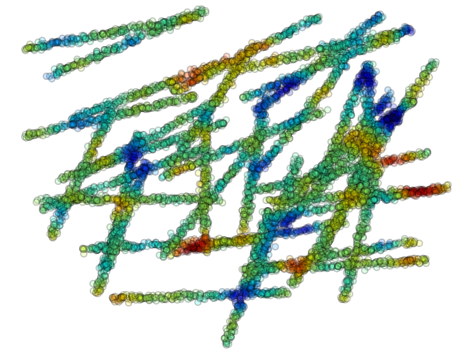
\includegraphics[width=\textwidth]{lines_truth}
                \caption{ Ground truth locations; color shows first of
                  50 output dimensions. The generative lengthscale is 1/20 the width of the
  image. }
                \label{fig:linestrue}
        \end{subfigure}\hspace{0.5em}
\begin{subfigure}[t]{.22\textwidth}
                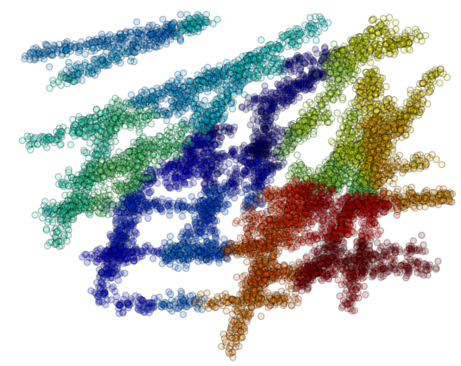
\includegraphics[width=\textwidth]{lines_init}
                \caption{Noisy observed locations, color shows
                  inference partition. (MAD=0.027)}
                \label{fig:linesinit}
        \end{subfigure}\hspace{0.5em}
\begin{subfigure}[t]{.22\textwidth}
                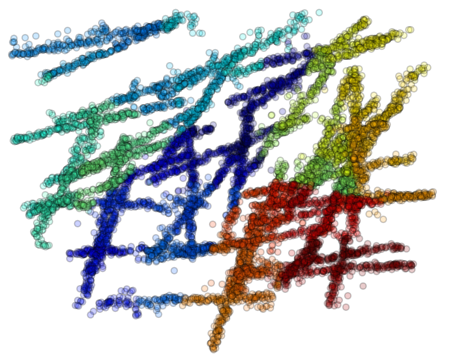
\includegraphics[width=\textwidth]{lines_local}
                \caption{Locations recovered by a local GP (L-200, MAD=0.0085). }
                \label{fig:lineslocal}
        \end{subfigure}\hspace{0.5em}
\begin{subfigure}[t]{.22\textwidth}
                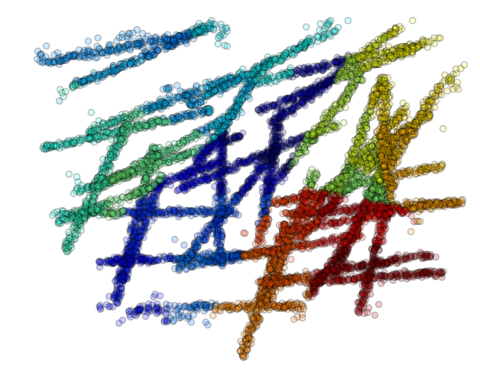
\includegraphics[width=\textwidth]{lines_gprf}
                \caption{ Locations recovered by a GP random field
                  (RF-200, MAD=0.0037).}
                \label{fig:linesgprf}
        \end{subfigure}
\caption{Synthetic line data consisting of 10000 points with noisily
  observed locations, each represented by a
  50-dimensional output ``waveform''. }
\label{fig:lines}
\end{figure}

\begin{figure}
    \centering
    \begin{minipage}{.45\textwidth}
        \centering
        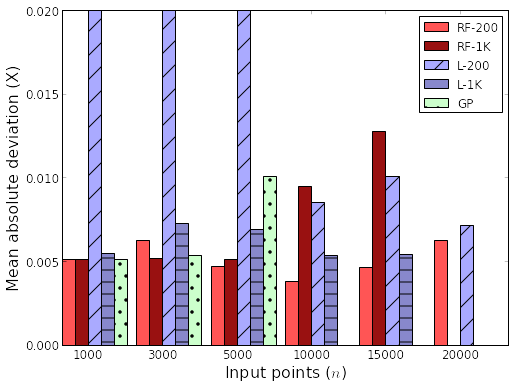
\includegraphics[width=\textwidth]{crazylines_half}
        \caption{Mean average deviations for local GPs (L) and GPRF (RF) with
          block sizes $m=200$ and $m=1000$, and for the full GP. The off-scale
          values for L-200 are approximately 0.08.}
        \label{fig:linesresults}
    \end{minipage}%
   \qquad
    \begin{minipage}{0.45\textwidth}
        \centering
        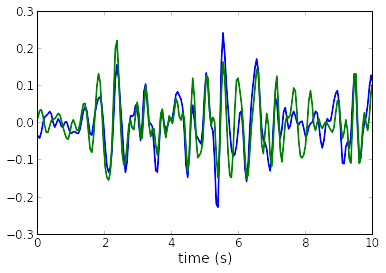
\includegraphics[width=\textwidth]{xcorr}
        \caption{Amplitude-normalized waveforms for two distinct seismic events
          occurring in the same region. Their reported locations
          are 29.5km apart; the true locations are likely much closer. \cite{ISCcitation2015} }
        \label{fig:wavematch}
    \end{minipage}
\end{figure}

To investigate the GPRF model, we created a family of 2D synthetic
datasets consisting of overlapping random lines of constant length,
intended to evoke a seismic fault structure. 
To generate a dataset of $n$ observations, we first sample $n/250$
random  lines in a square of width $\sqrt{n/1000}$, and for each line 
we sample $250$ points from a Gaussian tube with standard deviation 0.008. 
These are the ``ground truth''
event locations $X$; we generate ``waveforms'' $Y$ for these events by sampling
from a GP with 50 independent output dimensions, using a SE kernel
with lengthscale $0.15$ (Figure~\ref{fig:linestrue}). We then perturb the
true locations with isotropic Gaussian noise to generate a set of noisy
locations, $\hat{X} \sim \N(X, 0.2\cdot \mathcal{I})$. These noisy locations and
their generating distribution are treated as a prior on $X$ during
inference; we also use $\hat{X}$ as the initialization  (Figure~\ref{fig:linesinit}). 

We attempted to recover the true event locations using the full GP-LVM
model, local GPs (GP-LVM with block-diagonal covariance imposed) and
the GPRF, using blocks of size 200 and 1000. Partitions were chosen randomly
using the RPC method suggested by \cite{chalupka2012}, applied to the
noisy locations $\hat{X}$. We ran L-BFGS on each objective for two
hours or until convergence, whichever was sooner. As shown in
Figure~\ref{fig:linesresults}, the local GP models sometimes failed
entirely to converge to a reasonable solution, getting stuck in
faraway local minima. The GPRF models performed well, essentially
matching the full GP-LVM, and beating it at $n=5000$ when the two-hour
runtime limit started to become a constraint. For larger $n$, the
RF-1000 model also started to run out of time, yielding poor
performance, but RF-200 continued to outperform the local GPs. 

\begin{figure}
\centering
\begin{subfigure}[t]{.45\textwidth}
 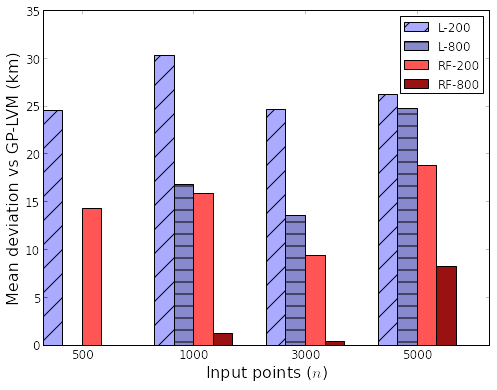
\includegraphics[width=\textwidth]{seismic_loc}
\caption{Mean deviations (in km) from GP-LVM locations on real seismic
  events (lower is better).}
\label{fig:seismicloc}
\end{subfigure}
\qquad
\begin{subfigure}[t]{.45\textwidth}
 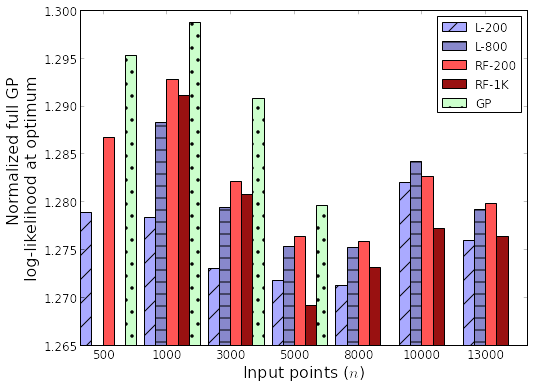
\includegraphics[width=\textwidth]{seismic_lik}
\caption{Full GP-LVM marginal likelihood (normalized by $nD$) at the
  recovered locations (higher is better).}
\label{fig:seismiclik}
 \end{subfigure}
\end{figure}
\vspace{-1em}
\subsection{Seismic data}
\vspace{-.5em}
We also evaluated on a real seismic dataset, consisting of 13,000 waveforms aligned with 
P wave arrivals at the Mankachi array (MKAR) in Kazakhstan
between  April 1, 2008 and
April 1, 2009. Each waveform is 10s long and sampled at 20Hz
($D=200$). Location prior information comes from the ISC event
bulletin \cite{ISCcitation2015}, which we use as initialization. 
Unlike in the synthetic case, there is no ground truth, so we compare 
the approximate algorithms against
GP-LVM. We subsample the dataset by picking a central
point and selecting the $n$ closest events, yielding smaller datasets
on which it is possible to run GP-LVM. Figure~\ref{fig:seismicloc}
shows the mean deviation, in kilometers, of the approximate locations from
the locations recovered by GP-LVM MAP inference. The approximate
models run for at most one hour, except on the full dataset ($n=2000$)
where they were run for two hours. Here the RF-800 model is very close
to exact inference, while the local GPs introduce significant
error. It is not feasible to run GP-LVM inference on the full dataset of 13000 events, but we can perform a single (very slow) computation
of the GP-LVM marginal likelihood on the final event hypothesis output
by each method, giving some measure of the quality of each method as a
surrogate (Figure~\ref{fig:seismiclik}). Although all methods struggled
with convergence at larger scales\footnote{Note to reviewers: a final
  version of this paper will evaluate these methods using longer
  runtimes, where we expect the fully-converged GPRF to maintain its
  dominance.}, on the full dataset the RF-200 model continued to outperform the local GPs,
operating in a regime where it would be impossible to run a full GP. 

\section{Conclusions and Future Work}
\vspace{-.5em}
The Gaussian process random field is a tractable and effective
surrogate for the GP marginal likelihood, evading a large intractable
computation by partitioning the data into smaller blocks. It has the flavor of
approximate inference methods such as loopy belief propagation, but
can be analyzed precisely in terms of a determinstic approximation to
the inverse covariance, and additionally provides a new training-time
interpretation to the Bayesian Committee Machine. It is easy to
implement and its evaluation can be straightforwardly parallelized. 

An issue left mostly undiscussed in this paper is the selection of the
partition itself. Most published work uses simple clustering
heuristics such as $k$-means \cite{tresp2000bayesian} or RPC
\cite{chalupka2012} on the $X$ values, but this is unsatisfying in the
latent variable setting where those values may be
unobserved. \cite{rasmussen2006} suggests that considering $\v{y}$ in
the partition may be helpful even for regression applications, but we
are unaware of any published work on doing so. 

Another useful avenue for future work would be the integration of the
GPRF framework with inducing point methods, similarly to the
integration of inducing points with local GPs accomplised by PIC \cite{snelson2007}.

%\section{Acknowledgements}
% DTRA grant. MSR grant. 
%

\bibliographystyle{unsrt}
\bibliography{refs}

\end{document}
